\documentclass[11pt, french]{report}

\usepackage[utf8x]{inputenc}
\usepackage[french]{babel}
\usepackage[T1]{fontenc}
\usepackage{amsmath}
\usepackage{vmargin}
\usepackage{listings}
\usepackage[usenames,dvipsnames]{color}
\usepackage{graphicx}
\usepackage{hyperref}
\usepackage[toc,acronym]{glossaries}
\makeglossaries

\setpapersize{A4}

\begin{document}

%%%%%%%%%%%%%%%%%%%%%%%%%%%%%%%%%%%%%%%%%%%%%%%%%%%%%%%%%%%%%%
%%%%%			DEBUT MISE EN FORME DE LA PAGE DE GARDE

\makeatletter
\def\clap#1{\hbox to 0pt{\hss #1\hss}}%
\def\ligne#1{%
\hbox to \hsize{%
\vbox{\centering #1}}}%
\def\haut#1#2#3{%
\hbox to \hsize{%
\rlap{\vtop{\raggedright #1}}%
\hss
\clap{\vtop{\centering #2}}%
\hss
\llap{\vtop{\raggedleft #3}}}}%
\def\bas#1#2#3{%
\hbox to \hsize{%
\rlap{\vbox{\raggedright #1}}%
\hss
\clap{\vbox{\centering #2}}%
\hss
\llap{\vbox{\raggedleft #3}}}}%

\def\maketitle{%
	\thispagestyle{empty}\vbox to \vsize{%
	\haut{}{\@blurb}{}
	\vfill
	\vspace{1cm}
	\begin{flushleft}
	\Huge \@title
	\end{flushleft}
	\par
	\hrule height 2pt
	\par
	\begin{flushright}
	\Large \@author
	\par
	\end{flushright}
	\vspace{1cm}
	\vfill
	\@logo
	\vfill
	\bas{}{Le \@date\\
	\vspace{1cm}
	\textbf{Tuteur :}\\
	Jean-Loup Guillaume \textit{(Université Pierre et Marie Curie)}	
	}{}	
	}%
	\cleardoublepage}

\def\date#1{\def\@date{#1}}
\def\author#1{\def\@author{#1}}
\def\title#1{\def\@title{#1}}
\def\location#1{\def\@location{#1}}
\def\blurb#1{\def\@blurb{#1}}
\def\logo#1{\def\@logo{#1}}
\author{}
\title{}
\location{}\blurb{}
\makeatother
\title{Projet tutoré\\ \textbf{Application Freepod pour iOS}}
\author{Adrien \textsc{Humilière}}
\location{Paris}
\blurb{%
\textbf{Université Pierre et Marie Curie (UPMC)}\\
Année universitaire 2011/2012\\
Licence de Sciences et Technologies, mention Informatique\\
Développeur d'Applications Nouvelles Technologies}% 
\logo{
	\begin{center}
		
\includegraphics[width=10cm]{logo_freepod.png}\\
	\end{center}
}
\maketitle

%%%%%%%%%%%%%%%%%%%%%%%%%%%%%%%%%%%%%%%%%%%%%%%%%%%%%%%%%%%%%%
%%%%%			FIN MISE EN FORME DE LA PAGE DE GARDE


%%%%%%%%%%%%%%%%%%%%%%%%%%%%%%%%%%%%%%%%%%%%%%%%%%%%%%%%%%%%%%
%%%%%			SOMMAIRE

\tableofcontents



%%%%%%%%%%%%%%%%%%%%%%%%%%%%%%%%%%%%%%%%%%%%%%%%%%%%%%%%%%%%%%
%%%%%			Glossaire
     								
\chapter*{Glossaire}
\addcontentsline{toc}{chapter}{Glossaire}

\paragraph{Podcast}

Le terme Podcast (né de la contraction des mots iPod et broadcast) désigne une méthode de diffusion de contenus multimédias (audio ou vidéo) sur Internet. Les fichiers sont diffusés par le biais de flux RSS 2.0. Ils peuvent ensuite être récupérés sur un appareil au moyen d’un aggrégateur.
La plupart des radios et certaines chaines de télévision diffusent leurs émissions en podcast. Existent également des émissions indépendantes, produites pour être diffusées sous forme de podcast (on parle ici de podcast indépendant).

\paragraph{Podcasteur}

Communément utilisé pour désigner une personne animant ou réalisant un podcast indépendant.

%%%%%%%%%%%%%%%%%%%%%%%%%%%%%%%%%%%%%%%%%%%%%%%%%%%%%%%%%%%%%%
%%%%%			INTRODUCTION
     								
\chapter*{Introduction}
\addcontentsline{toc}{chapter}{Introduction}

%%%%%%%%%%%%%%%%%%%%%%%%%%%%%%%%%%%%%%%%%%%%%%%%%%%%%%%%%%%%%%
%%%%%			Freepod et ses applications

\chapter{Freepod et ses applications}
\section{Présentation de Freepod et objectifs des applications mobiles}

Freepod est une association regroupant une quinzaine de podcasts indépendants sur différents thèmes (jeux-vidéo, hacking, culture japonaise, théâtre, politique, actualité technologique, etc.). Elle a été fondée en août 2011 et continue son chemin depuis, en intégrant de nouveaux podcasts et en leur proposant de nouveaux outils. L’auteur de ce rapport est co-fondateur et secrétaire de l’association.

L’objectif principal de Freepod est de mutualiser les moyens des podcasteurs pour diviser les coûts et simplifier la diffusion des émissions.
Pour cela, elle s’est dotée d’un site internet qui référence l’ensemble des émissions produites par les différents podcasts (depuis 2007) et permet de les écouter (pour les podcasts audio) ou de les visionner (pour les podcasts vidéo).

La nature du podcast et l'essor depuis quelques années de l’informatique mobile rendent indispensable le développement de solutions permettant d’écouter ou de visionner simplement des émissions en situation de mobilité. C’est pour cette raison que Freepod cherche aujourd’hui à se doter d’applications natives pour les principales plates-formes mobiles. 
Deux étudiants de notre promotion de L3 DANT sont impliqués dans le développement de ces applications : Michel Knoertzer pour la plate-forme Windows Phone 7 et moi-même pour la plate-forme iOS et le Web Service commun à toutes les plates-formes. Une déclinaison pour la plate-forme Android est également prévue.

\section{Fonctionnalités attendues}

Un cahier des charges (fourni en annexe) a été défini entre l’association et les développeurs, pour fixer les fonctionnalités attendues de l’application, même si elles ne sont pas toutes considérées comme indispensables dans un premier temps.

\paragraph{Écoute des podcasts audio et vidéo}

L’écoute et le visionnage devront pouvoir se faire en streaming sur une connexion WiFi ou 3G. Idéalement, l’application permet à l’utilisateur de télécharger une émission (par exemple sur un réseau) pour pouvoir l’écouter ou la visionner plus tard (sans ou avec une mauvaise couverture data).

\paragraph{Écoute des enregistrements en direct}

Freepod propose à ses auditeurs de suivre l’enregistrement des émissions en direct par internet. L’application devra permettre de suivre un flux audio de ces enregistrements en direct.

\paragraph{Notification des utilisateurs}

L’application devra notifier l’utilisateur quand une nouvelle émission est disponible sur l’application ou quand l’enregistrement d’une émission en direct commence.

\paragraph{Discussion en direct}

La discussion en direct est une plus value importante des enregistrements en direct. Elle permet aux auditeurs d'interagir entre eux et avec les animateurs. L’application devra proposer un système permettant de discuter en direct avec les autres utilisateurs, quelle que soit leur plate-forme (mobile ou web).

\subsubsection{Autres fonctionnalités possibles}

Les podcasts permettent une forte interaction entre les auditeurs et les animateurs. Elle passe notamment par les réactions aux émissions. L’application pourrait afficher pour chaque émission les commentaires laissés, voir proposer la publication de nouveaux commentaires.
Pour aider à la propagation des émissions, l’application pourrait inclure un système de partage de liens sur les réseaux sociaux (Twitter, Facebook, Google+).
Un onglet pourrait proposer une liste de tweets concernant l’association (via le hashtag \#freepod).
Pour simplifier la consultation des contenus “texte”, l’application pourrait également proposer une version web mobile du forum, ainsi que le contenu du blog et les photos les plus récentes.

\section{Architecture du projet (Web Service et application)}
Ce projet est décomposé en deux parties distinctes. 

D’une part, le développement d’un Web Service basé sur les technologies LAMP (pour Linux, Apache, MySQL, PHP), qui permettra aux applications de différentes plates-formes de récupérer les données des podcasts. 

D'autre part, le développement d'une application pour iPhone, répondant aux différentes fonctionnalités du cahier des charges.

\subsection{Le web-service}

Basiquement, un Web Service est un outil informatique permettant l'échange de données entre des applications situées sur des plateformes hétérogènes. Le Web Service propose une série de requêtes qui peuvent être exécutées par un client et, soit renvoie des données (dans un format exploitable), soit procède à des actions en interne.

\subsubsection{Principe}

Nous avons fait ici le choix de concevoir un Web Service sur lequel les applications pourront se connecter pour récupérer les données. 

Ce Web Service aura pour mission de récolter les informations dans les flux RSS des podcasts et de les stocker dans une base de données avant de les redistribuer aux applications. Il est rendu particulièrement indispensable par la difficulté de traitement de ces flux RSS. Peu de normalisation à ce niveau et chaque podcasteur a ses pratiques pour l'écriture du fichier XML et pour un même élément, 2, voir 3, écritures différentes peuvent exister. Mieux vaut donc effectuer ce traitement une seule fois pour toutes les plateformes plutôt que de le répéter dans chaque application.

Il permettra également de répondre à certains besoins de Freepod pour partager son contenu avec des sites partenaires.

\begin{figure}[!h]
	\begin{center}
	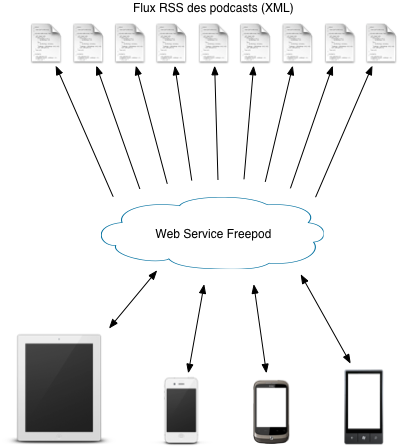
\includegraphics[width=8cm]{schema_webserv.png}
	\caption{\small{Schéma explicatif du fonctionnement du Web Service. Il récupère le contenu des fichiers XML des différents podcasts et les applications se connectent à lui pour récupérer les données.}} \label{webserv}
	\end{center}
\end{figure}

\subsubsection{Conception}

Pour le Web Service, nous allons nous baser sur un modèle de conception relativement simple. Il s'agit de lister les podcasts, et pour chaque podcast de lister les épisodes. Un podcast a un essentiellement un nom et un flux RSS (référençant les épisodes), mais nous pourrons y ajouter d'autres informations (images, URLs, etc.). Un épisode a un titre, une durée, une url vers le fichier (audio ou vidéo), une image, etc.

Parallèlement à ces tables "fondamentales", nous devrons gérer les logins et mots de passe des utilisateurs, ainsi que des statistiques de base (nombre de requêtes). Une telle base de données, selon le modèle entités/associations sera représentée comme indiqué dans le schéma ci-contre.

\begin{figure}[!h]
	\begin{center}
	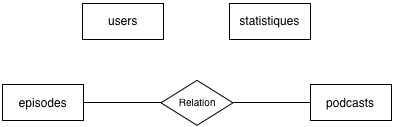
\includegraphics[width=8cm]{schema_entite_assoc.png}
	\caption{\small{Schéma Entités / Associations pour la base de données du Web Service Freepod}} \label{entiteAssoc}
	\end{center}
\end{figure}

\subsection{Application iOS}

Sur la plate-forme iOS, plus encore que sur d'autres systèmes, l'expérience utilisateur joue un rôle primordiale. La qualité du système conçu par Apple depuis 2007 et la très forte concurrence entre les applications sur l'App Store (500 000 applications disponibles, plus de 25 milliards d'applications téléchargées) font que les utilisateurs ne s'attardent pas sur une application mal conçue, lente, buggée ou dont l'ergonomie ne répond pas aux canons d'iOS.

\subsubsection{Conception}

Comme indiqué plus haut, l'application Freepod pour iOS aura pour vocation essentielle l'écoute des émissions produites par l'association. Pour la première étape de développement de cette application que constitue ce projet, j'ai choisi de me concentrer sur cette fonctionnalité et de ne développer les autres que si le temps le permet.

Une des premières étapes du projet a donc été de concevoir un diagramme de classe simplifié, qui serve de point d'appui pour le développement de l'application. De la même manière que l'architecture du web-service, celle de ce projet est relativement simple.

\begin{figure}[!h]
	\begin{center}
	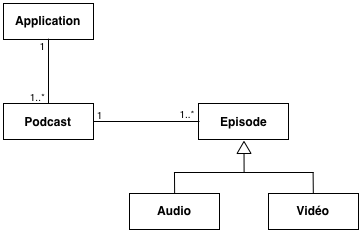
\includegraphics[width=8cm]{diag_class.png}
	\caption{\small{Diagramme de classes pour l'application Freepod iOS. \textit{Elaboré avant le début du développement de l'application.}}} \label{classes}
	\end{center}
\end{figure}

\subsubsection{Interfaces Homme-Machine}

Les interfaces homme-machine sont une des clés du développement sur iOS. Apple apporte d'ailleurs une attention particulière à ce que les développeurs respectent ses \textit{iOS Human Interface Guidelines} puisqu'il s'agit de l'un des principaux critères de validation des applications avant publication sur l'App Store qui permet de les distribuer.

J'ai donc dessiné une série de schémas de ma vision de l'application que j'ai pu soumettre aux membres de l'association pour obtenir leurs avis. En me basant sur ces retours, j'ai pu préparer les IHM présentées ci-contre, qui constituent les objectifs de design et d'interaction de l'application

\begin{figure}[!h]
	\begin{center}
	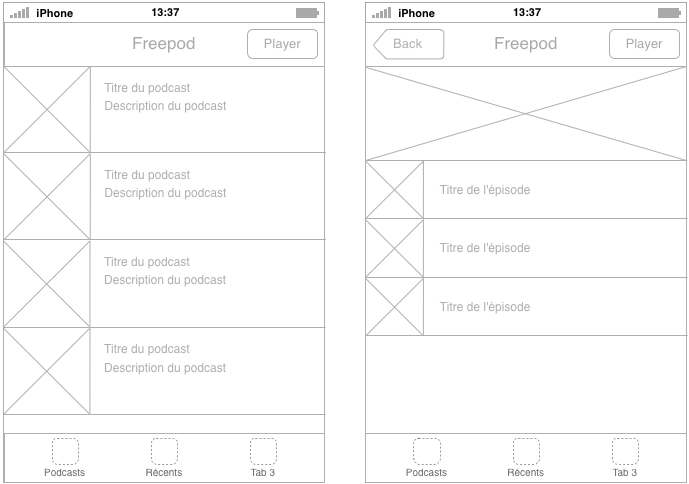
\includegraphics[width=12cm]{ihm_tableviews.png}
	\caption{\small{Interfaces homme-machine pour les principales vues de l'application Freepod. \textit{A gauche :} Interface pour la vue "Podcasts" qui liste l'ensemble des podcasts de l'application. \textit{A droite :} Interface pour la vue "Episodes" qui liste l'ensemble des épisodes pour un podcast donné.}} \label{classes}
	\end{center}
\end{figure}

\begin{figure}[!h]
	\begin{center}
	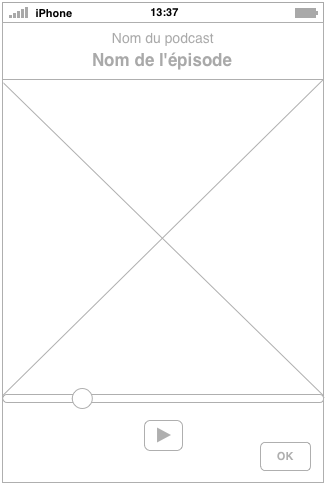
\includegraphics[width=5.6cm]{ihm_player.png}
	\caption{\small{Interfaces homme-machine pour les principales vues de l'application Freepod. \textit{Ici :} Interface pour la vue "Player" qui affiche l'illustration d'un épisode et permet de contrôler la lecture.}} \label{classes}
	\end{center}
\end{figure}



%%%%%%%%%%%%%%%%%%%%%%%%%%%%%%%%%%%%%%%%%%%%%%%%%%%%%%%%%%%%%%
%%%%%			Le SDK iOS et Objective-C

\chapter{Le SDK iOS et Objective-C}

iOS est le système d’exploitation mobile développé par Apple pour fonctionner sur iPhone, iPad et iPod Touch. Il est dérivé de Mac OS X (basé sur UNIX). Apple propose aux développeurs enregistrés un SDK (Software Development Kit) qui permet de développer des applications pour iOS avec le langage Objective-C.

Dans cette partie, nous allons présenter Objective-C, puis le SDK iOS, le framework CocoaTouch et les outils de développement fournis par Apple, qui fournissent un environnement de travail complet. 

\section{Présentation d'Objective-C}

\subsection{Historique}

Le langage Objective-C est créé au début des années 80 par Brad Cox. L'inventeur le met au point en se basant sur le langage Smalltalk-80 et le destine à être une surcouche du C du C permettant la programmation orientée objet.

En 1989, sort le système d'exploitation NeXTSTEP qui est le premier à utiliser Objective-C. NeXTSTEP est l'OS développé par la société NeXT qui fut fondée par Steve Jobs lors de son éviction d'Apple.

Lors du rachat de NeXT par Apple en 1996, ses ingénieurs se servent de NeXTSTEP comme noyau de base pour ce qui deviendra quelques années plus tard Mac OS X. L'Objective-C est également utilisé dans iOS, lui même basé sur MAC OS X.

La compilation de l'Objective-C se fait avec GCC (GNU Compiler Collection).

\subsection{Spécificités du langage}

Parce qu'Objective-C est dérivé du C, une grande partie des propriétés du langage en dépendent.

Il présente cependant un certain nombre de spécificités, par exemple par rapport à d'autres langages orientés objet comme le C++ lui aussi directement dérivé du C :
\begin{itemize}
	\item La distribution dynamique des messages permet à chaque message de déclencher une partie de code différente à l'exécution en fonction du type du destinataire. Le langage décide dynamiquement de la manière de traiter un message à partir de la classe du destinataire.
	\item Objective-C permet de choisir entre le typage statique ou dynamique. C'est-à-dire que le développeur peut choisir que le type de l'objet soit défini à la compilation ou à l'exécution.
	\item Le langage dispose enfin d'un mécanisme de chargement dynamique. C'est à dire que les composants du langages utilisés dans un programme en Objective-C sont chargés au fur et à mesure des besoins pendant l'exécution.
\end{itemize}

Par ailleurs, l'héritage multiple est impossible en Objective-C et toutes les classes héritent (directement ou indirectement) de la classe racine \verb NSObject . On ne parle pas de méthodes, mais de messages, transmis à un objet, dont la syntaxe est la suivante : \verb [object  \verb message] .

\section{Le SDK iOS}

Comme la plupart des langages de programmation, les bibliothèques intégrées à Objective-C sont insuffisantes pour programmer efficacement. C'est pour cette raison que le langage est très fortement lié à Cocoa (API native pour le développement sur Mac OS X \& iOS) ou à son pendant libre GNUstep.\\

Apple organise un réseau de développeurs baptisé \textit{Apple Developer}. Il est conçu pour rendre disponibles un certain nombre de ressources aux développeurs. Par ce programme, Apple met à disposition la documentation complète d'Objective-C, d'iOS et de Mac OS X, ainsi que les outils permettant de développer pour ces plateformes, comme Xcode 4.

Une partie de ces ressources est libre d'accès, mais le programme gratuit ne permet pas d'accéder aux pré-versions d'iOS, ni d'exécuter ses applications sur un appareil pour les tester.

\subsection{Bibliothèques iOS}

Le SDK (Kit de Développement Logiciel) iOS contient un certain nombre d'outils permettant la conception et la publication d'application pour iPhone, iPod Touch et iPad. Il est divisé en quatre composants : Cocoa Touch, Media / Application Services, Core Services et Core OS / Mac OS X kernel.

Il requiert pour fonctionner au minimum un Macintosh avec un processeur Intel.

\paragraph{Cocoa Touch} C'est le framework de plus haut niveau du SDK. C'est cette couche qui permet de gérer l'interface utilisateur. Elle permet également de gérer les fonctions multitâche et les contrôles tactiles de l'écran.

\paragraph{Couche Media} Cette couche contient les composants permettant la gestion des images (redimensionnement, transformation, etc.), de l'audio, de la vidéo (lecture, enregistrement) et des animations 3D.

\paragraph{Core Services} Permet la gestion du réseau et des threads. Cette couche contient aussi les outils de géolocalisation et une base de données locale de type SQLite.

\paragraph{Kernel} C'est la couche de plus bas niveau du SDK. Elle permet aux développeurs d'utiliser le protocole TCP/IP, les  sockets et le système de fichiers.

\subsection{Xcode 4}

Xcode est l'Environnement de Développement (IDE) proposé par Apple pour le développement d'application Mac OS X et iOS. Il est distribué clé en main avec les différents SDK et le compilateur GCC.

Il inclut tout ce qu'on peut attendre d'un éditeur de code, ainsi qu'une interface de type WYSIWYG pour la mise en place des interfaces Homme-Machine.


%%%%%%%%%%%%%%%%%%%%%%%%%%%%%%%%%%%%%%%%%%%%%%%%%%%%%%%%%%%%%%
%%%%%			Développement, limites du projet et évolutions futures

\chapter{Développement, limites du projet et évolutions futures}

\section{Le développement de l’application}

Le développement du Web Service et de l'application s'est fait en deux vagues. Dans un premier temps, au mois de février, j'ai développé l'essentiel du Web Service, afin de pouvoir commencer par la suite le développement des applications : celle pour la plate-forme Windows Phone 7 réalisée par Michel Knoertzer et celle pour iOS réalisée par moi-même dans un second temps au mois de mai.

\subsection{Le Web Service}

Pour cette première phase de développement que constitue le Web Service, j'ai choisi de n'aborder que les quatre points qui me semblaient particulièrement intéressants à détailler.

Le Web Service a été développé avec PHP et MySQL sur le serveur de l'association Freepod, un serveur dédié de type LAMP. Il est accessible à cette adresse : http://webserv.freepod.net (authentification nécessaire).

\subsubsection{Synchronisation de la base de données avec les flux RSS}

L'outil permettant de synchroniser la base de données avec les flux RSS des différents podcasts est le composant essentiel et le plus délicat de ce Web Service. C'est pour cette raison que j'ai choisi de m'y atteler en premier.\\

\lstset{language=XML, basicstyle=\ttfamily, keywordstyle=\color{blue}\bfseries, commentstyle=\color{JungleGreen}}

Comme indiqué précédemment, les flux RSS des podcasts (en fait un simple fichier XML) ne sont pas bien harmonisés chaque podcasteurs utilise ses propres outils pour les mettre en place. Certains utilisent des CMS les générants automatiquement, d'autres les génèrent à partir d'un logiciel dédié, d'autres encore éditent le code XML à la main. Cette diversité induit une diversité dans le code. L'inclusion d'une image pour un épisode se fait par exemple de deux manières différentes :
\begin{lstlisting}
<itunes:image href="http://url_image"/>
<itunes:image>http://url_image</itunes:image>
\end{lstlisting}
D'autres épisodes ne spécifient tout simplement pas d'image et il faut alors remplacer dans la base de données par l'image par défaut du podcast. Cette partie use donc d'un grand renfort de boucles conditionnelles.\\

Pour maintenir la synchronisation entre les flux RSS et la base de données (certains épisodes pouvant être supprimés ou modifiés), je me suis basé sur la comparaison de la date et l'heure de publication, ainsi que sur la chaine de cratères du nom. Un épisode ne dispose pas d'identifiant unique dans les flux, et cette méthode permet aux podcasteurs de modifier les informations de leurs podcasts dans la base de données simplement, en modifiant la date ou le nom d'un épisode.

Pour maintenir cette synchronisation sans intervention humaine, une tache CRON a été mise en place sur le serveur qui exécute le script de synchronisation toutes les 10 minutes.

\subsubsection{Les méthodes GET}

La méthode GET, bien qu'étant un composant essentiel du Web Service est relativement simple. Elle récupère les paramètres donnés dans l'URL et renvoie les données présentes en base après les avoir formatées en JSON.\\

Trois types de requêtes existent :
\begin{itemize}
	\item Récupération de la liste complète des podcasts
	\item Récupération de la liste des épisodes pour un podcast donné en paramètre
	\item Récupération de la liste des épisodes récents, dont le nombre est donné en paramètre
\end{itemize}


\subsubsection{La gestion des images}

\subsubsection{Interface d'administration}




\subsection{L'application pour iOS}

\subsubsection{Classes métier et récupération des données du Web Service}

\subsubsection{Navigation dans l'application}

\subsubsection{Lecture Audio et Vidéo}

\section{Limites}

\subsection{Difficultés rencontrés}



\subsection{Fonctionnalités non-implémentées}


\section{Evolutions futures}

\subsubsection{Développement d'un module de chat cross-plateformes}

\subsubsection{Télécharger pour écouter plus tard}

%%%%%%%%%%%%%%%%%%%%%%%%%%%%%%%%%%%%%%%%%%%%%%%%%%%%%%%%%%%%%%
%%%%%			CONCLUSION

\chapter*{Conclusion}
\addcontentsline{toc}{chapter}{Conclusion}



 
%%%%%%%%%%%%%%%%%%%%%%%%%%%%%%%%%%%%%%%%%%%%%%%%%%%%%%%%%%%%%%
%%%%%%%%%%%%%%%%%%%%%%%%%%%%%%%%%%%%%%%%%%%%%%%%%%%%%%%%%%%%%%
%%%%%			DEBUT DES ANNEXES
%%%%%%%%%%%%%%%%%%%%%%%%%%%%%%%%%%%%%%%%%%%%%%%%%%%%%%%%%%%%%%
%%%%%%%%%%%%%%%%%%%%%%%%%%%%%%%%%%%%%%%%%%%%%%%%%%%%%%%%%%%%%%

\part*{Annexes}
\addcontentsline{toc}{part}{Annexes}

\appendix

\chapter{Applications Freepod - Cahier des charges}

Freepod est une association qui regroupe une douzaine de podcasts indépendants. Elle propose un portail web pour que ces podcasts se fassent connaître et pour regrouper la communauté sur un même lieu.

L’association cherche a proposer des applications pour faciliter l’écoute et le visionage de ses émissions sur des plateformes mobiles.\\

L’application devra donc contenir les fonctionnalités suivantes, par ordre de priorité :

\paragraph{Écoute des podcasts audio et vidéo}
L’écoute et le visionage devront pouvoir se faire en streaming sur une connexion wifi ou 3G. Idéalement, l’application permet à l’utilisateur de télécharger une émission pour pouvoir l’écouter plus tard.

\paragraph{Écoute des enregistrements en direct}
Freepod propose à ses auditeurs de suivre l’enregistrement des émissions en direct par internet. L’application devra permettre de suivre ce flux audio en direct.

\paragraph{Notification des utilisateurs}
L’application devra notifier l’utilisateur quand une nouvelle émission est disponible à l’écoute ou quand l’enregistrement d’une émission en direct commence.

\paragraph{Discussion en direct}
La discussion en direct est une plus value importante des enregistrements en direct. Elle permet aux auditeurs d'interagir entre eux et avec les animateurs. L’application devra proposer un système permettant de discuter en direct avec les autres utilisateurs, quelle que soit leur plateforme.\\

D’autres fonctionnalités pourront être ajoutées mais ne sont pas considérées comme indispensable par Freepod :
\begin{itemize}
\item Affichage pour chaque émission des commentaires aussi présents sur le site internet de Freepod. Publication de nouveaux commentaires depuis l’application.
\item Partage de liens vers les émissions sur les réseaux sociaux (Twitter, Facebook et Google+).
\item Affichage des tweets concernants Freepod.
\item Consultation du forum de Freepod.
\item Affichage du contenu du blog.
\item Affichage des photos concernant Freepod disponibles sur Flickr.
\item Lien vers la boutique de l’association.
\end{itemize}

\chapter{Mode d'emploi du l'interface web d'administration}




\chapter{Documentation du Web Service}



%%%%%%%%%%%%%%%%%%%%%%%%%%%%%%%%%%%%%%%%%%%%%%%%%%%%%%%%%%%%%%
%%%%%			BIBLIOGRAPHIE

\bibliographystyle{abbrv}
\nocite{*}
\addcontentsline{toc}{chapter}{Bibliographie}
\bibliography{biblio}

\end{document}
